\documentclass[a4paper,12pt,spanish]{article}
\usepackage[spanish,activeacute]{babel}
\usepackage[utf8]{inputenc}
\usepackage{tocbibind}
\usepackage[colorlinks=true,linkcolor=blue]{hyperref}
\usepackage{eurosym}
\usepackage{listings}
\usepackage{color}
\usepackage{fancyvrb}
\usepackage{times}
\usepackage{sans}

\newcommand{\urltilde}{$_{\widetilde{~}}$}

\definecolor{gray95}{gray}{.95}
\definecolor{gray85}{gray}{.85}
\definecolor{gray45}{gray}{.45}

\lstset{ frame=Ltb,
     framerule=0pt,
     aboveskip=0.5cm,
     framextopmargin=3pt,
     framexbottommargin=3pt,
     framexleftmargin=0.4cm,
     framesep=0pt,
     rulesep=.4pt,
     backgroundcolor=\color{gray95},
     rulesepcolor=\color{black},
     %
     stringstyle=\ttfamily,
     showstringspaces = false,
     basicstyle=\footnotesize\ttfamily,
     commentstyle=\color{gray45},
     keywordstyle=\bfseries,
     %
     numbers=left,
     numbersep=15pt,
     numberstyle=\tiny,
     numberfirstline = false,
     breaklines=true,
}

\lstdefinelanguage{Groovy}
{keywords={abstract,any,as,boolean,break,byte,case,catch,char,class, 
const,continue,def,default,do,double,else,extends,false,final,finally, 
float,for,goto,if,implements,import,instanceof,in,int,interface,label, 
long,native,new,null,package,private,protected,public,return,short, 
static,strictfp,super,switch,synchronized,this,throw,throws,transient, 
true,try,void,volatile,while,with}}

\lstset{language=Groovy,
	tabsize=2,
	basicstyle=\footnotesize,
	keywordstyle=\color{black}\bfseries,
	identifierstyle=,
	commentstyle=\color{blue},
	stringstyle=\ttfamily,
	showstringspaces=false,
	sensitive=true,% 
	morecomment=[l]//,% 
	morecomment=[s]{/}{/},% 
	morestring=[b]",% 
	morestring=[b]',%
}		

% minimizar fragmentado de listados
\lstnewenvironment{listing}[1][]
   {\lstset{#1}\pagebreak[0]}{\pagebreak[0]}

\lstdefinestyle{consola}
   {basicstyle=\footnotesize\bf\ttfamily,
    backgroundcolor=\color{gray85},
    rulesep=0pt
   }
 
\lstdefinestyle{Java}
   {language=Java,
   }

\lstdefinestyle{html}
   {language=html,
   }

\lstdefinestyle{Groovy}
   {language=Groovy,
   }


\RequirePackage{ifpdf} % ¿latex o pdflatex?
% Configuración de las imágenes
\ifpdf
	\usepackage[pdftex]{graphicx}	% Inclusión de imágenes
	\DeclareGraphicsExtensions{.pdf,.png,.jpg}
\else
	\usepackage{graphicx}		% Inclusión de imágenes
	\DeclareGraphicsExtensions{.eps}
\fi
\graphicspath{ {./img/} } % Ruta respecto al fichero tex principal dónde se buscan

\oddsidemargin 0in
\textwidth 6.5in
\topmargin -0.5in
\textheight 9.5in
\parindent 0em

\usepackage{charter,helvet}
\usepackage{a4wide,fancyhdr}
\usepackage{color,array,graphicx}

\definecolor{p308}{cmyk}{1,0,0,0.51}
\definecolor{p152}{cmyk}{0,0.51,1,0}
\definecolor{pcg9}{cmyk}{0,0,0,0.65}

\newcommand{\lv}{\color{p152}\vline}
\setlength{\arrayrulewidth}{1pt}
\setlength{\extrarowheight}{-1ex}

\fancyhf{}
\setlength{\headheight}{50pt}

\lhead
{
  \footnotesize
  \begin{tabular}{@{}p{5cm}}
        
\includegraphics[height=12ex]{uca/uca}
  \end{tabular}
}

\chead
{
%
}

\rhead
{
  \footnotesize
  \begin{tabular}{!{\lv}p{3.5cm}}
    \color{pcg9}
    Ingeniería Web               \newline
    \color{p308}
    Ingeniería Informática       \newline
%    \mbox{}                                 \newline
    \mbox{}
  \end{tabular}
%  \footnotesize
%  \begin{tabular}{!{\lv}p{5cm}}
%    \color{pcg9}
%    Escuela Superior de Ingeniería          \newline
%    C/ Chile, 1. 11002 Cádiz                \newline
%    \makebox[2em]{Tel.\hfill} 956\,01\,5138 \newline
%    \makebox[2em]{Fax \hfill} 956\,01\,5139
%  \end{tabular}
}

\renewcommand{\headrulewidth}{0pt}
\renewcommand{\footrulewidth}{0pt}

\pagestyle{fancy}


\author{Ingeniería Web -- Universidad de Cádiz}
%\author{Adrián Cepillo Macías}
\title{Tutorial de Introducción a Grails}

\begin{document}
\begin{titlepage}
  \maketitle
  \begin{figure}[h!]
    \centering
    \vspace{0.2in}
    
\includegraphics[scale=0.35]{grailsportada}
    \label{fig:Portada}
  \end{figure}
  \tableofcontents
\end{titlepage}
 

\newpage 

\section{Instalación de Grails}

En este tutorial vamos a instalar Grails manualmente. Primero descargar la aplicacion desde \href{http://grails.org/Download}{grails.org}. La extraemos en el directorio que deseemos, por ejemplo en el directorio \urltilde/grails.\\

Luego hay que definir una variable de entorno:
\begin{listing}[style=consola]
$ export GRAILS_HOME=~/grails/bin
\end{listing}

Podemos hacer esto permanente introduciendo este comando al final del fichero  \urltilde/.bashrc.\\

Aunque en este tutorial no usaremos grails por consola, se muestra esta instalación por si se necesita usar grails independientemente de Eclipse STS. Veremos en este tutorial algunos de los comandos que grails contiene para generar el esqueleto de una aplicacion web, probarla, etc. Todo ello lo haremos desde el {\it prompt} que nos ofrece Eclipse STS.

\section{Creando una aplicación}

Vamos a crear de nuevo la aplicación que maneja libros. Creamos un nuevo proyecto y esta vez elegiremos una instalación específica de Grails, en lugar de la que viene incluida en Eclipse STS. Para ello debemos pulsar en {\it Configure Grails Installations} y añadir la versión de Grails que acabamos de descargarnos, indicando el directorio en el que se encuentra.\\

\begin{centering}
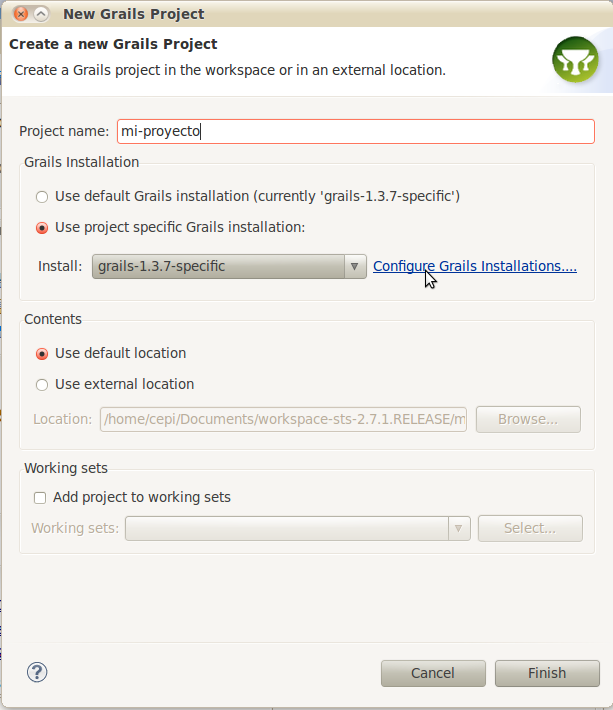
\includegraphics[scale=0.35]{new-project}\\
\end{centering}

{\bf Nota:} El comando de {\it Grails} para crear un proyecto es:
\begin{listing}[style=consola]
$ grails create-app mi-proyecto
\end{listing}

Eclipse STS no permite crear un nuevo proyecto introduciendo este comando en el prompt.\\

Para conocer algunos de los comandos de {\it Grails} vamos a usar el prompt que nos presenta {\it Eclipse STS}. Podemos encontrarlo en Navigate$\rightarrow$Open Grails Commands Prompt, pinchar en el simbolo de {\it Grails} en la barra de herramientas o pulsar Ctrl+Alt+Shift+G (Cmd+Alt+Shift+G en Mac). Con Ctrl+Space (Cmd+Space) nos mostrará el asistente de comandos posibles a ejecutar.\\

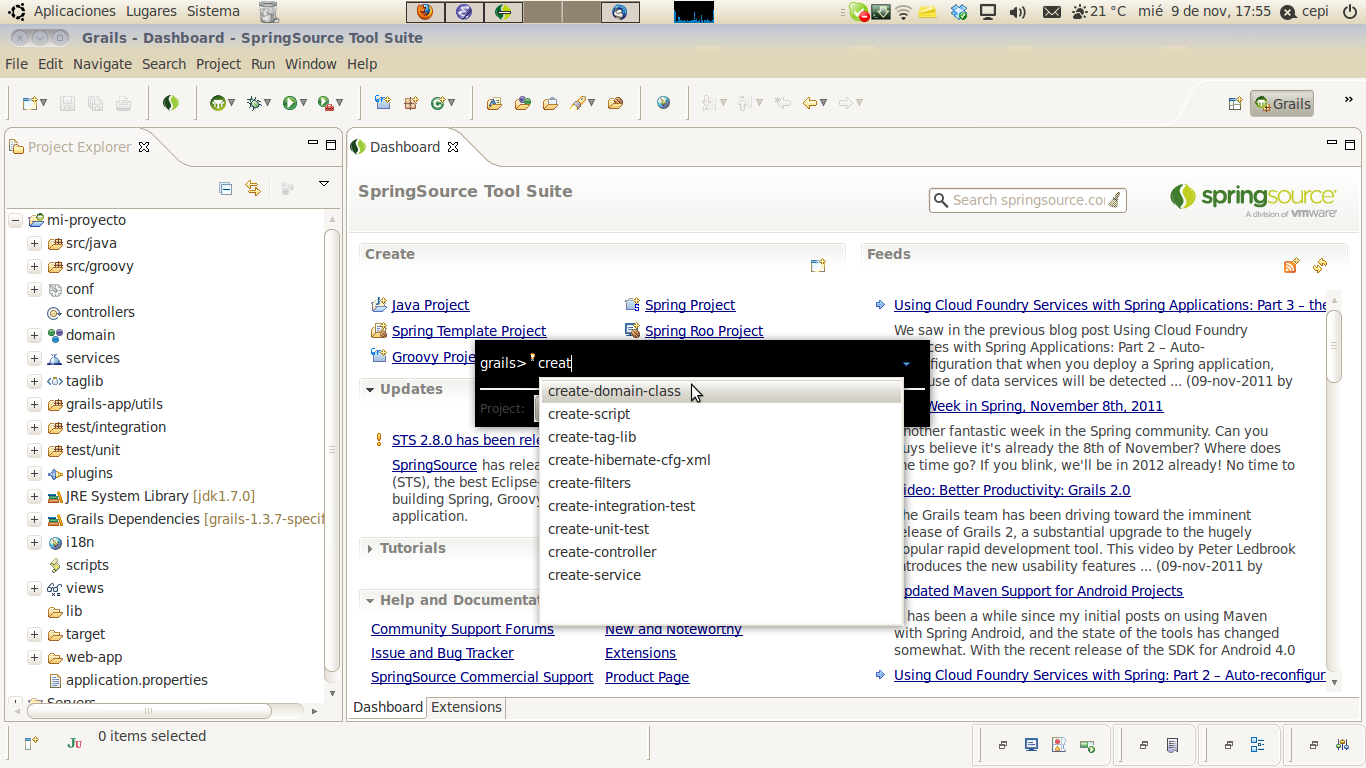
\includegraphics[scale=0.35]{create-domain}\\

Ahora crearemos la clase de dominio introduciendo en el prompt:
\begin{listing}[style=consola]
grails> create-domain-class org.example.Book
\end{listing}

Modificamos el código:\\

\lstinputlisting[style=Groovy]{resources/Book.groovy}

Y lo mismo para el controlador:

\begin{listing}[style=consola]
grails> create-controller org.example.Book
\end{listing}


\lstinputlisting[style=Groovy]{resources/BookController.groovy}

Ejecutamos la aplicación mediante:

\begin{listing}[style=consola]
grails> run-app
\end{listing}

Hasta ahora hemos hecho lo mismo que el tutorial anterior de Eclipse STS, pero pidiéndole al scaffolding de Grails que nos genere distintos componentes de la aplicación web por nosotros.

\section{Creando datos \textit{mock} de prueba}

Es probable que queramos probar la aplicación con ciertos datos \textit{mock} (simulados) y sería muy pesado tener que introducirlos a mano cada vez que se ejecutara la aplicación. Para ello modificaremos el fichero de configuración {\it BootStrap.groovy}, dentro de {\it conf} en la jerarquía del proyecto.

\lstinputlisting[style=Groovy]{resources/BootStrap.groovy}

Con esto hemos redefinido {\it init} en el Servlet controlador principal de la aplicación. De esta forma cada vez que se inicie la aplicación se crearán estos datos como ejemplares del modelo.\\ 

Debemos notar la llamada a {\it Book.count()}. Este método devuelve el número de libros que existen ya en la base de datos. Con el {\it if()\{...\}} decimos que en caso que no existan otros datos de testeo, se introduzcan estos datos.\\

Por otra parte, para cada instancia de {\it Book} llamamos al método {\it Book.save()}, el cual guarda el objeto en la base de datos. En la llamada definimos la opción {\it failOnError: true} indicando que se lance una excepción en caso que el método falle.

\section{Configuración del Data Source}

Hasta ahora hemos estado trabajando con la base de datos por defecto que emplea Grails, HSQLDB. Esta es una base de datos guardada en memoria principal, que sirve principalmente para desarrollo y pruebas. Vamos a configurar una base de datos alternativa. Para ello modificamos el fichero {\it DataSource.groovy}.

\lstinputlisting[style=Groovy]{resources/DataSource.groovy}

En este caso estamos usando {\it MySql} a través del framework de persistencia {\it Hibernate}. El fichero DataSource.groovy define tres orígenes de datos diferentes para una misma aplicación: desarrollo, pruebas y producción.

Grails ya dispone de drivers para JDBC, pero es necesario descomentar varias líneas del fichero {\it BuildConfig.groovy}.

\lstinputlisting[style=Groovy]{resources/BuildConfig.groovy}

\section{Ampliando nuestra aplicación}
\subsection{Creando la clase Author}

Vamos a añadir algunos elementos nuevos a la aplicación, empezando por crear otra clase de dominio llamada {\it Author} que se relacione con {\it Book}. Se muestra primero el código de la {\it domain class}:

\lstinputlisting[style=Groovy]{resources/Author.groovy}

Y por otra parte el controlador:

\lstinputlisting[style=Groovy]{resources/AuthorController.groovy}

\subsection{Relaciones entre clases con GORM}

Ahora vamos a crear una relación 1:N unidireccional entre Author y Book. Para ello modificamos la clase {\it Author}:

\lstinputlisting[style=Groovy]{resources/AuthorGORM.groovy}

En el caso de la clase {\it Book} no es necesario modificarla. Si la navegabilidad entre Book y Author fuera bidireccional, habría que añadir la siguiente línea de código a la clase Book:

\begin{listing}[style=Groovy]
static belongsTo = [author:Author]
\end{listing}

%\lstinputlisting[style=Groovy]{resources/BookGORM.groovy}

%\subsection{Modificando un controlador generado}

%%% Los controladores generados que he visto estan compilados.

\subsection{Cambio de estilo en la vista}

Grails genera una hoja de estilo por defecto que se encuentra en el directorio {\it mi-proyecto/web-app/css/main.css}. En el siguiente documento hemos modificado el color de los enlaces y los encabezados $<$h1$>$.

%Más adelante se mostrará como crear nuevas vistas con GSP y se añadiran nueva hojas de estilos.

\lstinputlisting[style=html]{resources/main.css} 

\end{document}
